%! TEX root = ../main.tex
\documentclass[../main.tex]{subfiles}

\begin{document}

\subsection{Fenditura $\mathbf{\qty{0.02}{\mm}}$}

Per la fenditura da $\qty{0.02}{\mm}$ ed apertura del sensore pari a $\qty{1.5}{\mm}$ sono stati raccolti $4$ set di dati che sono riportati in \autoref{fig:single scatter 0.02}.

\begin{figure}[ht!]
    \centering
    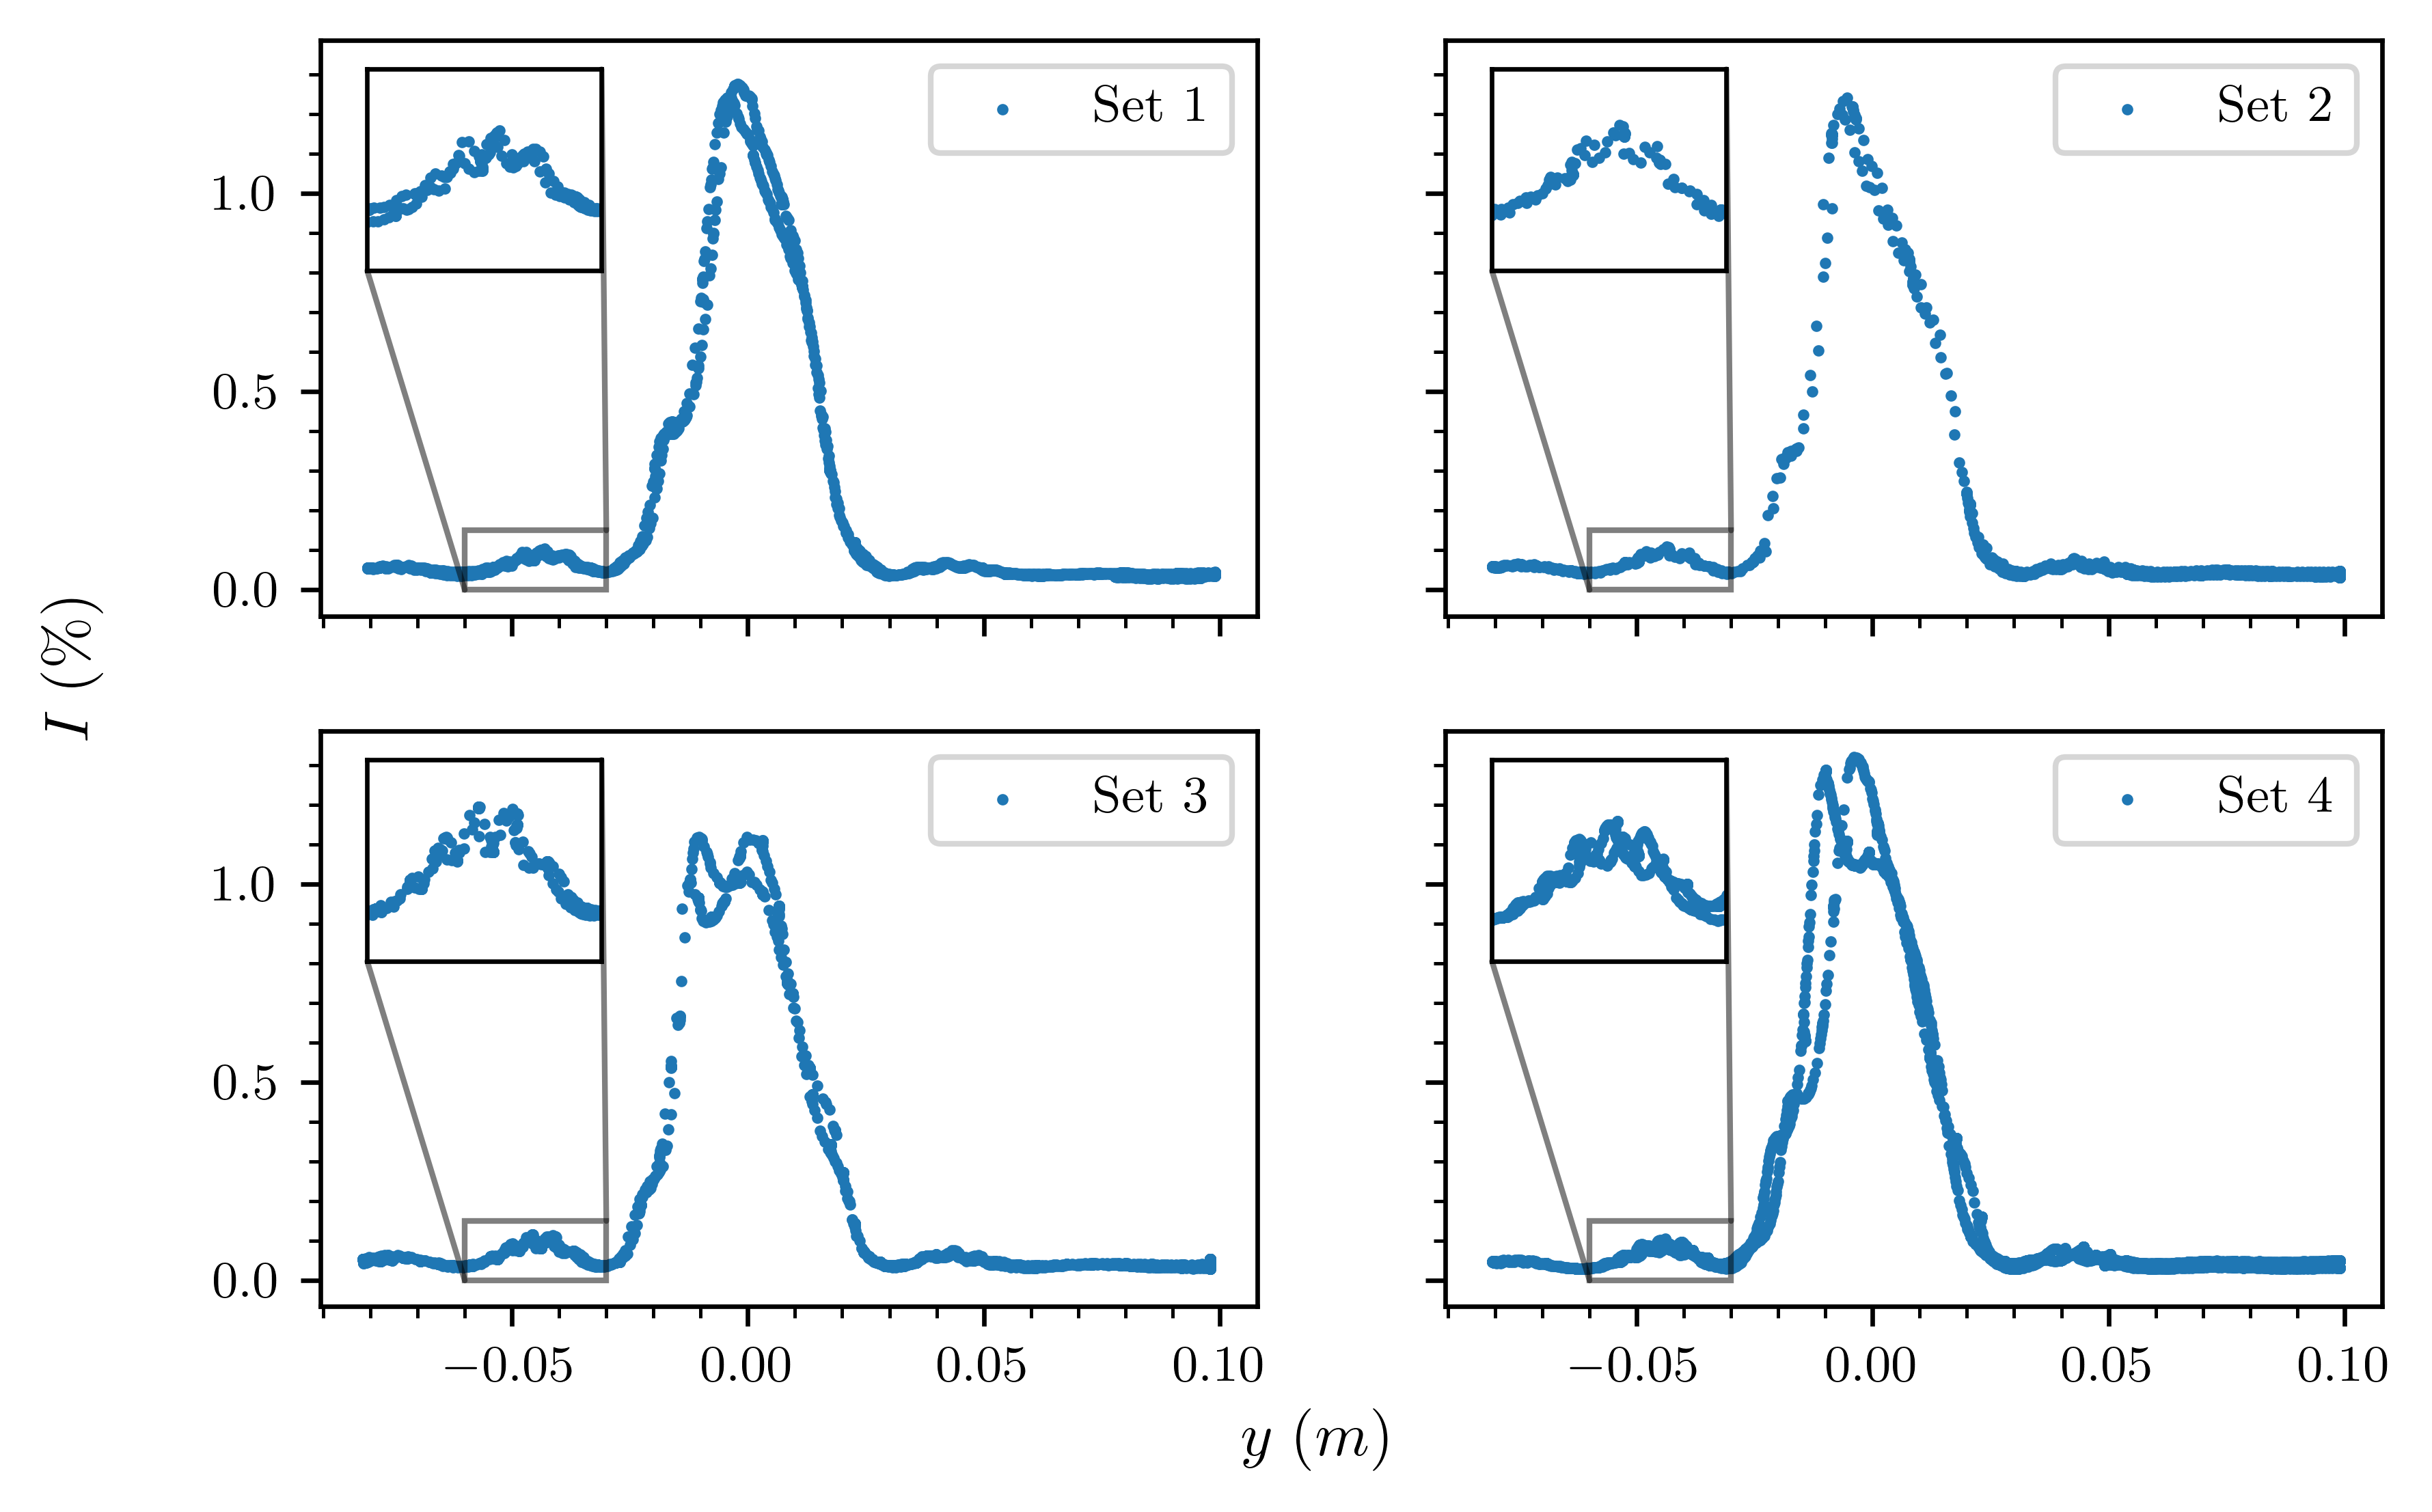
\includegraphics{single_scatter_0.02.png}
    \caption{Misure dell'intensità luminosa $I$ in funzione della posizione $y$ (in metri) del sensore. In tutti i set è possibile notare una deformazione del picco centrale che tende verso sinistra; a partire dal picco centrale del Set $3$ si può ipotizzare la presenza di un segnale sinusoidale che si sovrappone alla figura di diffrazione causando la biforcazione del picco centrale. La presenza di un segnale "parassita" è visibile anche nelle code della curva come mostrato nello zoom del picco laterale sinistro. Infine è presente un'asimmetria nelle code per cui l'intensità luminosa risulta essere maggiore a sinistra.}
    \label{fig:single scatter 0.02}
\end{figure}

Sovrapponendo i set si è proceduto ad individuare la posizione dei minimi attribuendogli una barra d'errore sufficientemente grande da rendere la misura compatibile con tutti i set. Le posizioni dei minimi ottenute dalla \autoref{fig:minimi 0.02} sono riportate in \autoref{tab:minimi 0.02} di fianco ai valori della fenditura ricavati utilizzando l'\autoref{eq:y=0 values}.

\begin{figure}[ht!]
    \centering
    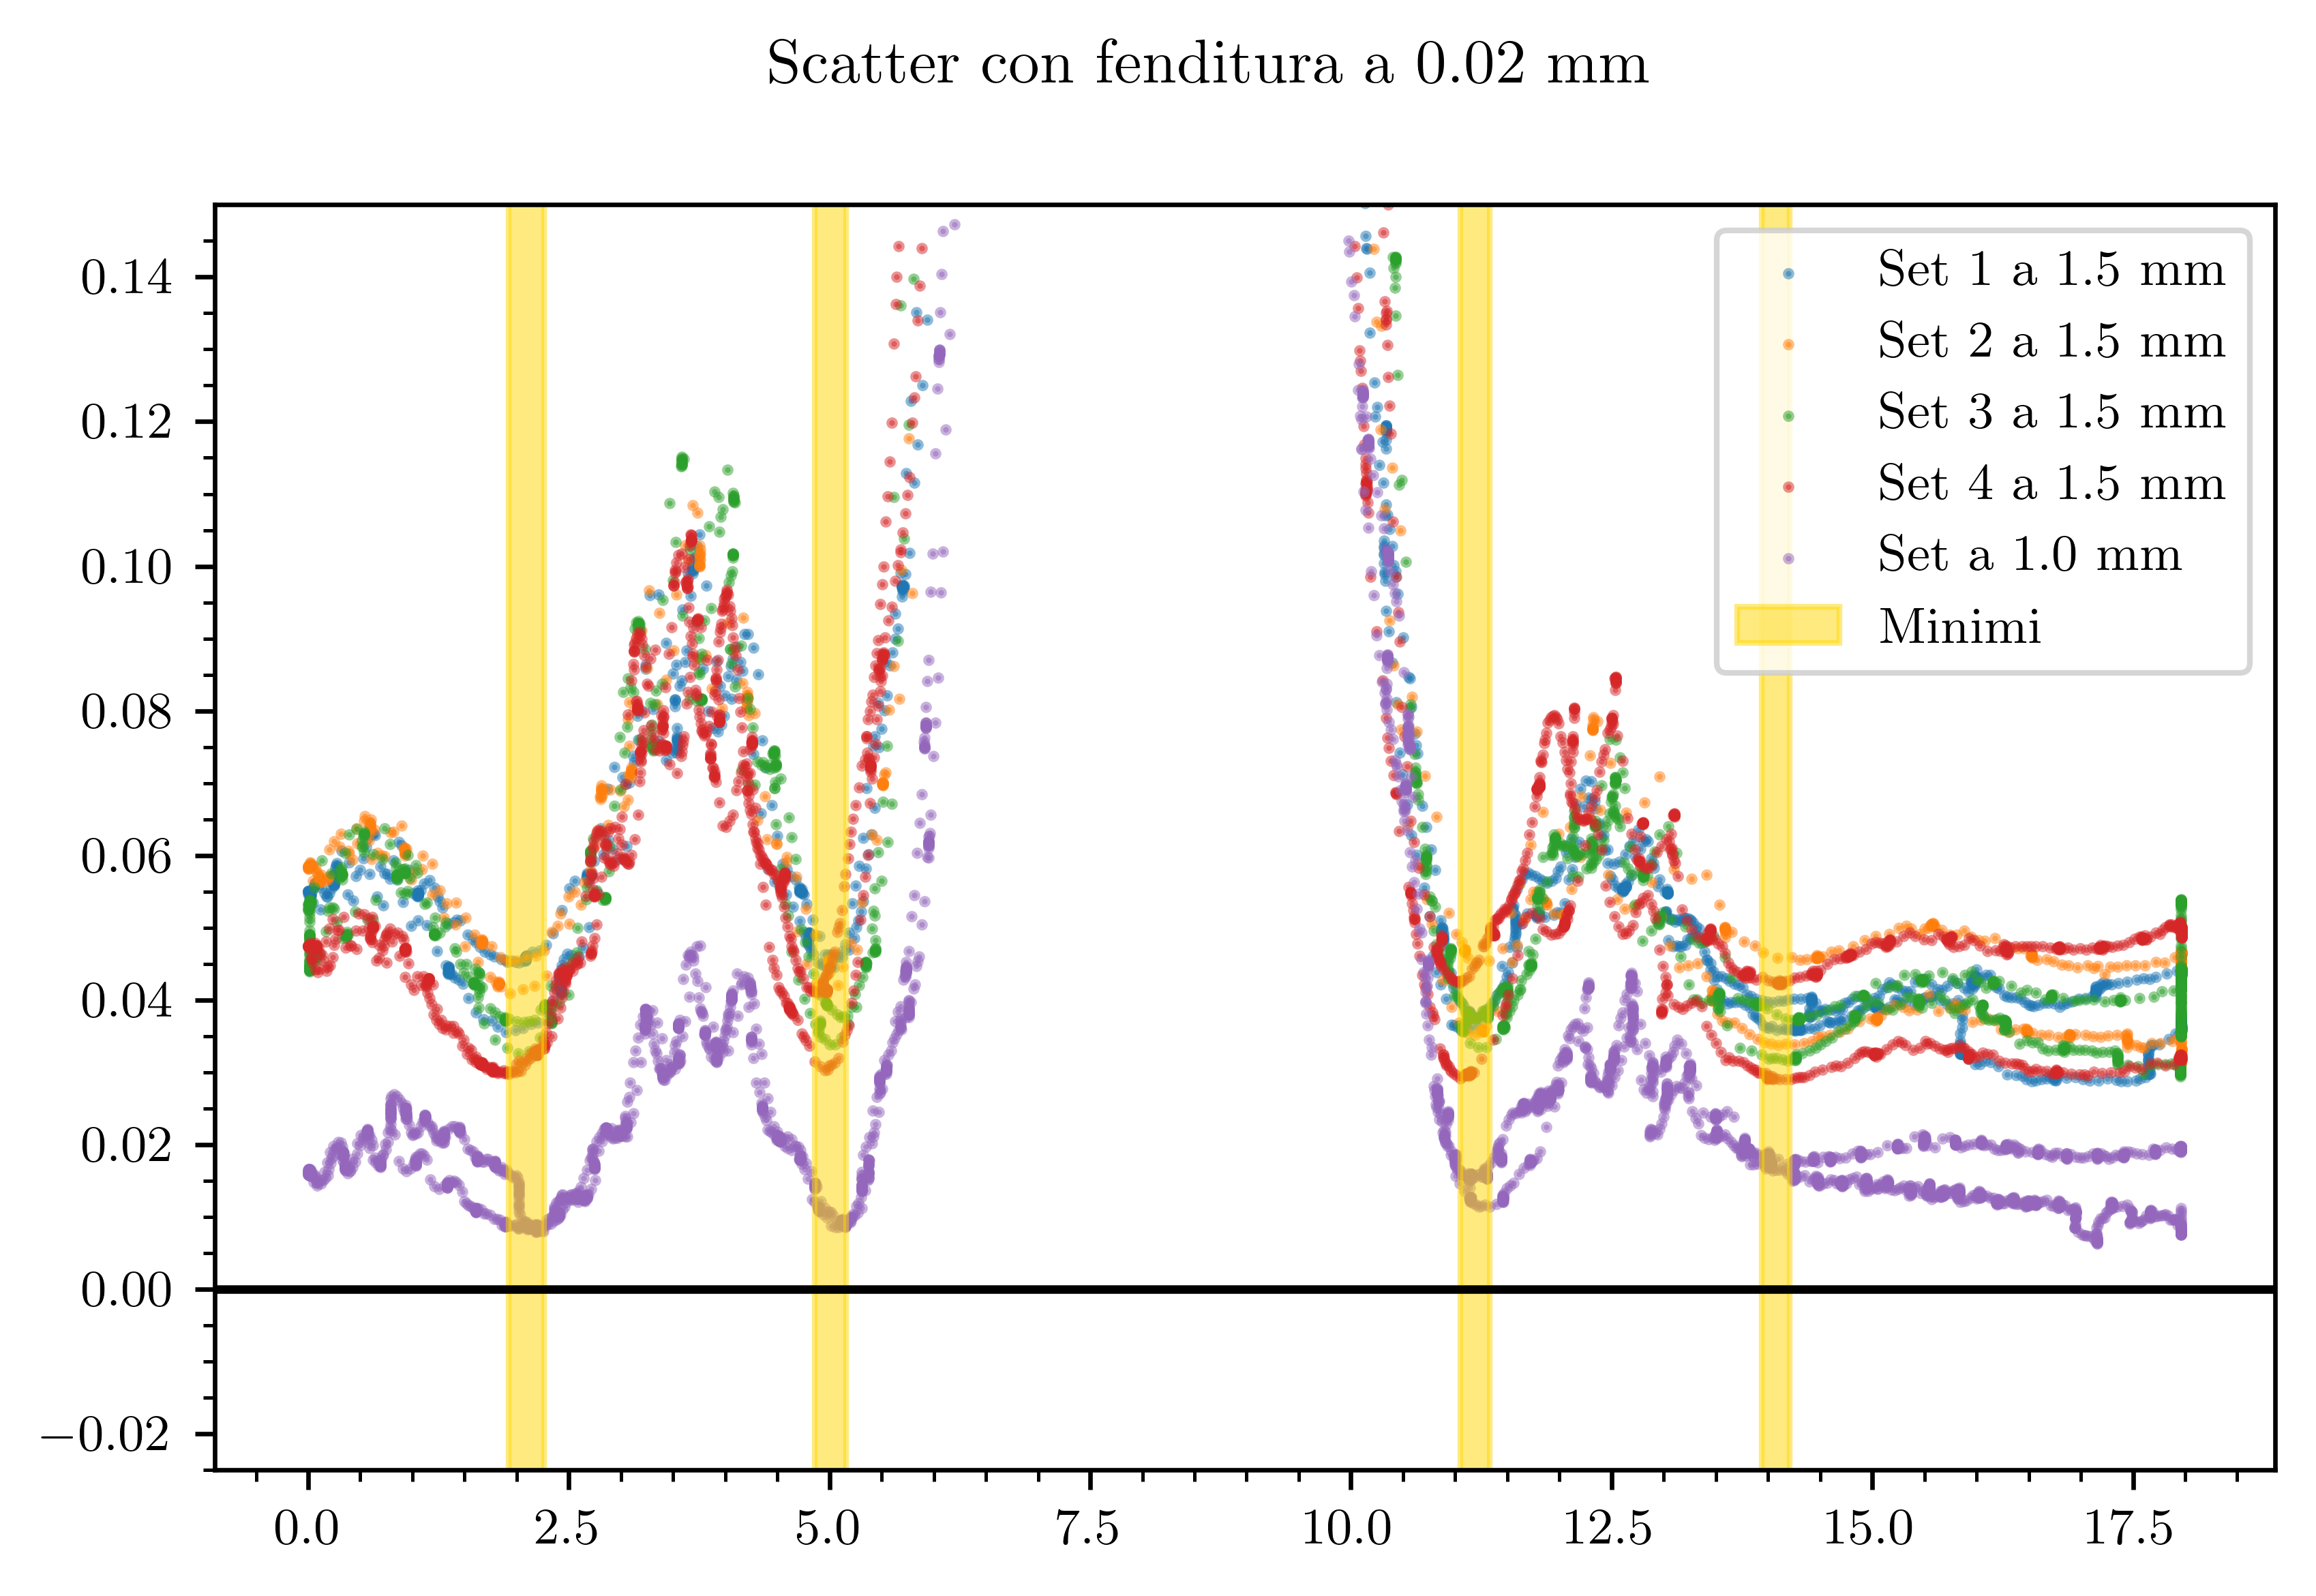
\includegraphics{min_0.02.png}
    \caption{Intensità luminosa $I$ in funzione della posizione $y$ del sensore (in metri) per la fenditura a $\qty{0.02}{\milli\metre}$. In figura sono segnati i minimi ricavati graficamente con i relativi errori. È possibile notare un segnale sinusoidale che si sovrappone alla figura di diffrazione causando una deformazione dei picchi laterali i quali risultano essere asimmetrici rispetto al centro, infatti l'intensità luminosa $I$ è inferiore per valori positivi della posizione.
        % Su ciascun minimo si considera un errore di posizione di $\qty{1.0}{\mm}$, che contribuisce all'ampiezza di ciascuno degli intervalli evidenziati. È possibile notare un segnale a frequenza costante che si sovrappone alla figura di diffrazione.
    } % todo: aggiungere qualcosa in più alla descrizione
    \label{fig:minimi 0.02}
\end{figure}

\begin{table}[ht!]
    \centering
    \caption{Posizione dei minimi, ottenuta graficamente dalla \autoref{fig:minimi 0.02}, riportata di fianco al proprio indice $m$ ed al valore $a$ (in $\si{\mm}$) stimato seguendo la relazione esposta in \autoref{eq:y=0 values}. Il valore di $a$ derivato da ciascun minimo è stato ricavato ponendo $\lambda = \qty{650}{\nm}$ ed $L = \qty{98.5+-0.1}{\cm}$. Per l'errore $\delta a$ sono stati sommati in quadratura $\delta y$ e $\delta L$, che permette di considerare trascurabile il contributo di $\delta L$.} %? review: fa un pò schifo l'ultima frase, ma il concetto è quello
    %? magari così va meglio? -v
    \import{../tables/}{mins_0.02.tex}
    \label{tab:minimi 0.02}
\end{table}

Intersecando le barre d'errore degli $a$ così ricavati si ottiene $a_g = \qty{0.021+-0.002}{\mm}$ che risulta compatibile con il valore teorico.

% Facendo una media pesata dei valori di $a$ ottenuti si ottiene $a = \qty{0.0209+-0.0012}{\mm}$. %? review: è meglio l'intersezione o la media?

\newpage

Successivamente si è proceduto con il fit utilizzando l'\autoref{eq:fit} e ottenendo un valore della fenditura $a_f = \qty{0.021+-0.002}{\mm}$, il grafico del fit è riportato in \autoref{fig:fit 0.02}.

\begin{figure}[ht!]
    \centering
    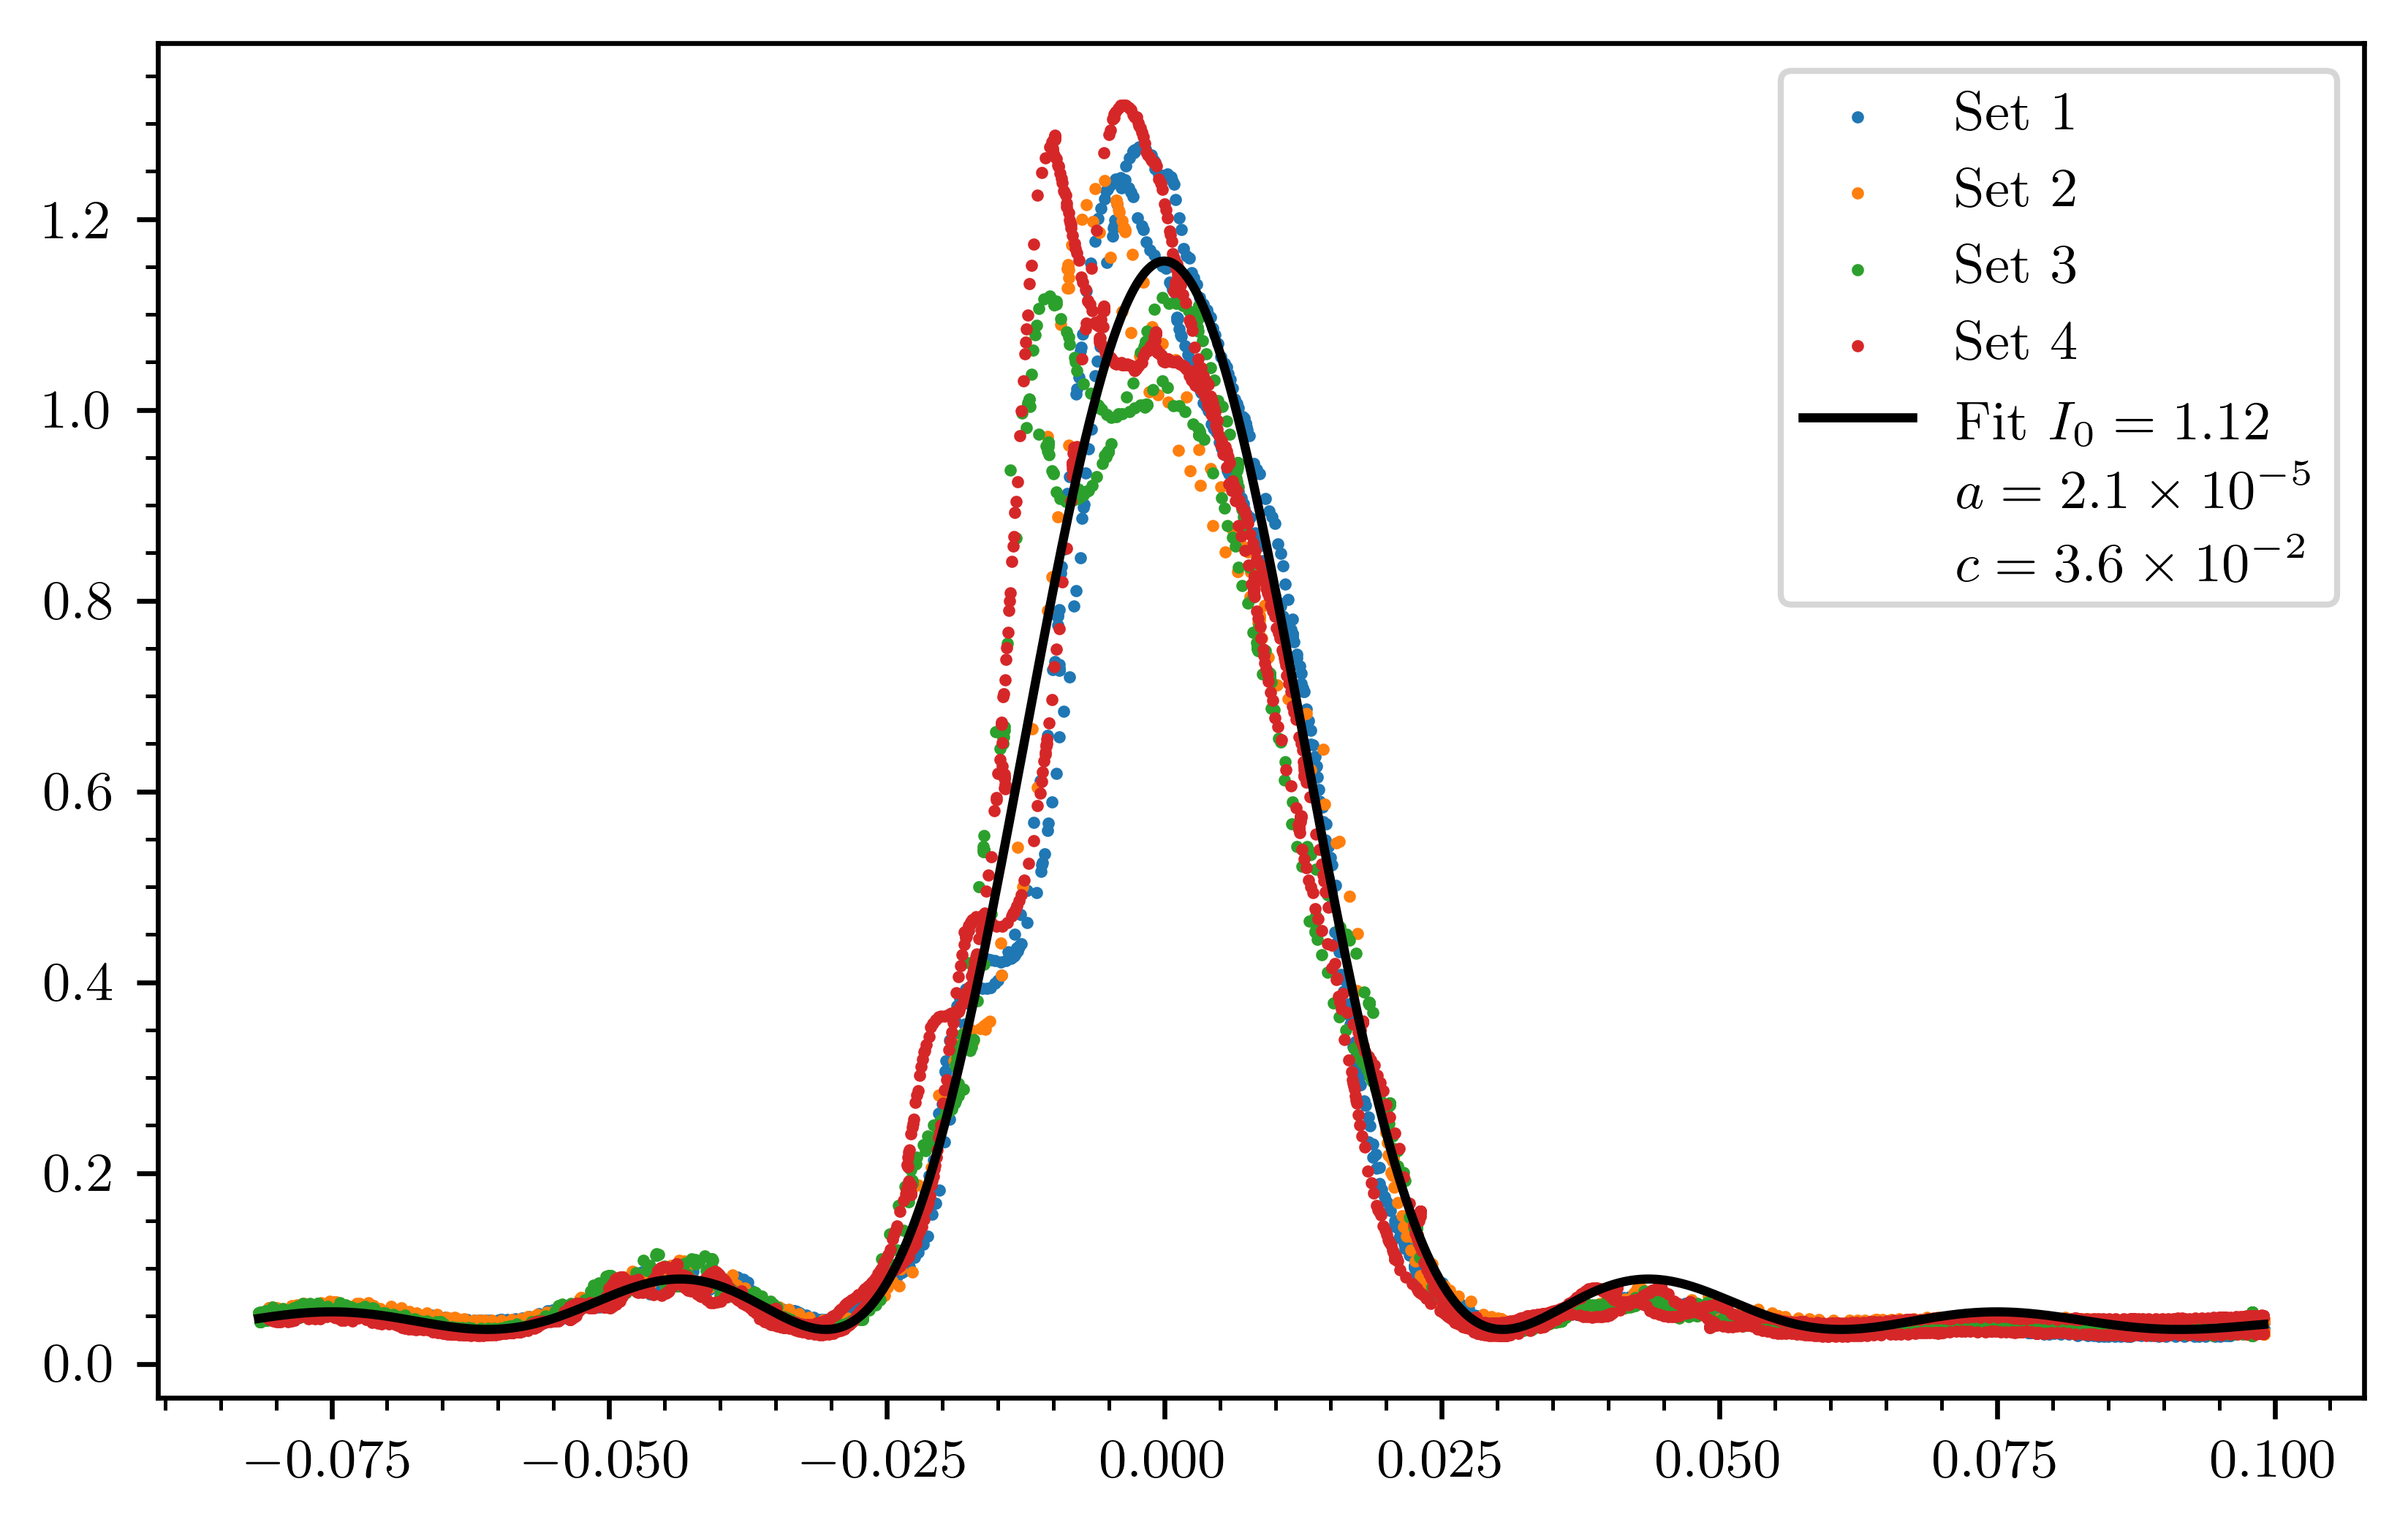
\includegraphics{fit_0.02.png}
    \caption{Intensità luminosa $I_{0}$ in funzione della posizione $y$ del sensore (in metri) per la fenditura a $\qty{0.02}{\mm}$. In figura è riportato il fit fatto utilizzando l'\autoref{eq:fit}. I valori dei parametri ottenuti sono $I_{0} = \num{1.12+-0.15}$, $a = \qty{0.021+-0.002}{\mm}$ e $c = \num{3.6+-0.8e-2}$.}
    \label{fig:fit 0.02}
\end{figure}

Entrambi $a_g$ e $a_f$ risultano compatibili con il valore teorico di $a = \qty{0.02}{\mm}$.

\newpage

Per confrontare le misure ottenute con diverse aperture del sensore si è scelto di utilizzare il set $1$, corrispondente alle misure con apertura $\qty{1.5}{\mm}$, in quanto è quello che meno presenta deformazioni lungo il picco centrale: questo permette un miglior confronto dell'ampiezza. Dopo aver scalato le intensità dei set utilizzati in modo che il valore massimo di $I$ risultasse pari ad $1$ per tutti i set, essi sono stati riportati sovrapposti in \autoref{fig:sensore 0.02}.

\begin{figure}[ht!]
    \centering
    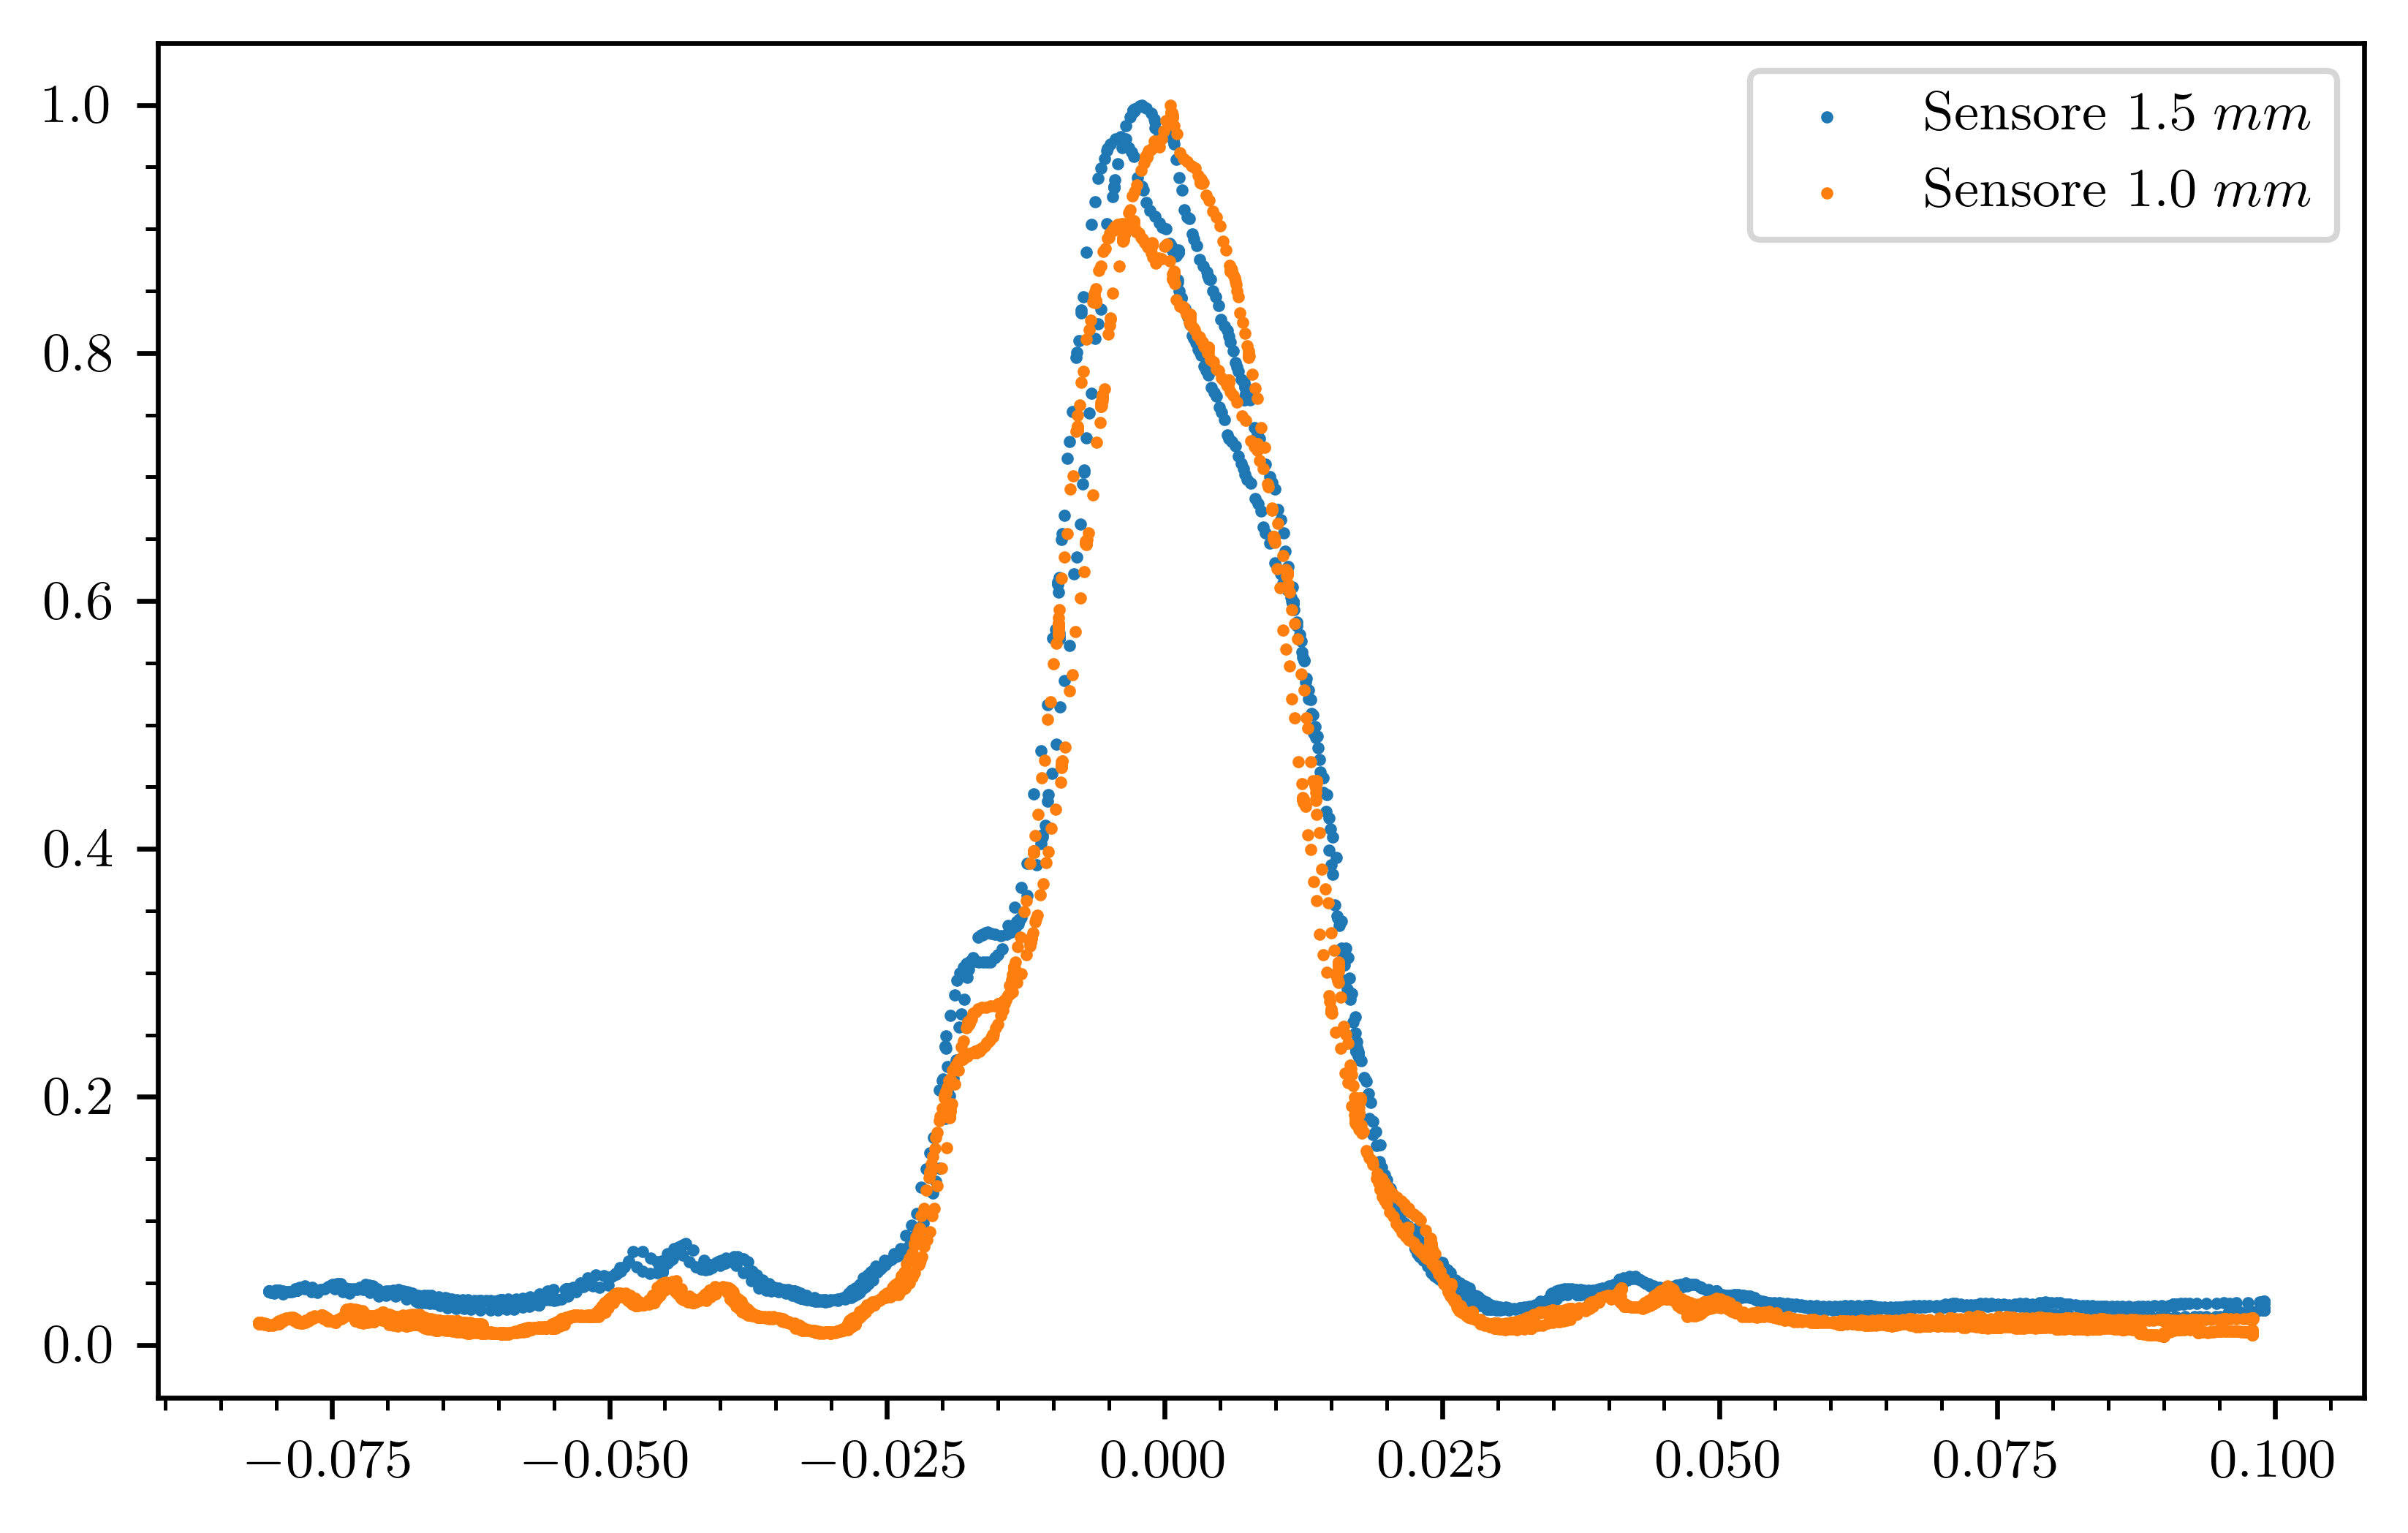
\includegraphics{sensor_0.02.png}
    \caption{Grafico dell'intensità luminosa relativa $I$ in funzione della posizione $y$ (in metri) per ciascuna delle due aperture del sensore.
        Riducendo l'apertura del sensore l'intensità misurata diminuisce permettendo di passare al fondo-scala più piccolo (\textit{candela}) per l'apertura da $\qty{1.0}{\mm}$.
        I valori delle intensità sono stati scalati in modo che l'altezza del picco centrale fosse pari a $1$, permettendo di confrontare i picchi con più semplicità. È possibile notare come la curva tracciata dalle misure con un'apertura più stretta abbia un picco centrale leggermente più schiacciato, tuttavia questo potrebbe essere dovuto ad un fattore di scala errato per l'intensità di una delle due curve in quanto esse non presentano un'intensità del picco centrale netta.
        Inoltre nelle code delle curve è evidente come il rumore di fondo diminuisca notevolmente, in particolar modo nel set di dati con il sensore a $\qty{1.0}{\mm}$. Questo potrebbe essere dovuto alla riduzione della luce che entra nel sensore o al cambio di fondo-scala, che porta ad una corrente di buio notevolmente inferiore. %? review: ha senso confrontare il rumore DOPO aver scalato i valori delle intensità?
        %* è probabile che sia un po' "banale" come considerazione, alla fine se scali il set contenente il rumore, giustamente il rumore subisce lo stesso cambio di scala, però conoscendo la vetri magari vuole lo stesso il commento, fa brodo
        Come sarà possibile vedere in seguito la seconda ipotesi è quella che più si adatta ai dati raccolti.} %! quantificare di quanto si stringe il picco
    \label{fig:sensore 0.02}
\end{figure}

Si può notare che anche nel grafico \ref{fig:sensore 0.02} persiste il segnale parassita: questo potrebbe essere dato da un difetto della fenditura stessa, che causa un'interferenza la quale si sovrappone alla figura di diffrazione.


\end{document}